\documentclass{article}
\usepackage[utf8]{inputenc}
\usepackage[french]{babel}
\usepackage[T1]{fontenc}
\usepackage{xspace}
\usepackage{listings}
\usepackage{xcolor}
\usepackage{graphicx}

\title{La réussite des alliances}
\author{Amine Mohammed ROSTANE et Gaillor Jowardo JINORO}
\date{02 Mai 2022}

\begin{document}
\maketitle
\tableofcontents

\section{Introduction}

\hspace{\parindent} Le langage Python est le premier des langages informatiques les plus utilisés dans le monde en 2022. Dans le cadre de ce projet, nous créons un jeu de cartes appelé: "La réussite des alliances". L'objectif principal de ce projet est de mettre en pratique toutes les connaissances que nous avons acquises durant le premier semestre.Par ailleurs, ce travail a été réalisé en binôme durant lequel les échanges se sont faits par l'outil de travail à distance "GIT" qui  est un outil efficace pour pouvoir collaborer à distance et mieux gérer les versions de code que l'on a implémenté.
\par Afin de voir plus clair dans ce qu'on a fait, nous divisons ce rapport en trois parties: tout d'abord, nous présenterons la généralité du jeu; ensuite, nous expliquerons nos implémentations des fonctions de la partie guidée du devoir; finalement, nous entamerons sur les extensions et les améliorations que nous avons apportées à ce sujet.


\section{Règles du jeu}

\hspace{\parindent} Avant tout, on nous a imposé l'unanimité sur le codage des cartes; c'est-à-dire que dans toute la logique du programme, une carte est représentée par un \emph{dictionnaire} ayant \textbf{deux clés: "valeur"} et \textbf{"couleur"}. Les valeurs sont par exemple: 2,3,A,Q,\ldots et les couleurs sont:  T(trèfle),K(carreau),C(coeur),P(Pique).

\par Par contre, on aimerait faire savoir dès le début qu'on a porté une légère modification à ce dictionnaire dans la partie "amélioration" histoire de se faciliter les tâches, lorsqu'on parlera de l'interface graphique. Désormais, voyons ci-dessous les règles du jeu et son déroulement:
\\
\begin{itemize}
  \item Le jeu se joue avec 32 ou 52 cartes.
  \item Après avoir choisi le nombre de cartes, il faut les battre.
  \item On choisit le nombre maximal de tas(pile de cartes) final, c'est-à-dire que si l'on dépasse ce nombre, la partie est perdue sinon, on gagne.
  \item Piocher une-à-une jusqu'à avoir au début 3 cartes que l'on pose de \textbf{gauche} à \textbf{droite}
  \item On dit qu'il y a saut ou bien un saut est possible si 2 tas séparés d'un autre tas au milieu, ont les mêmes couleurs ou mêmes valeurs. Si c'est le cas, ce tas du milieu va s'empiler au-dessus de celui d'avant(c'est aussi simple que ça!)
  \item S'il n'y a plus de saut possible on pioche une carte, on vérifie si un nouveau saut est possible et ainsi de suite,...
  \item Le jeu se termine lorsqu'on a fini toute la pioche ou bien que l'on a abandonné
  \item Le jeu est gagné si l'on a atteint le nombre maximal fixé au début ou encore moins(c'est mieux, et le coup parfait c'est de terminer avec 2 tas)
  \item Si le joueur a abandonné, c'est une défaite directe \\
\end{itemize}
\par Nous venons donc de comprendre les règles du jeu. En se basant sur celles-ci, nous avons pu nous créer des idées sur nos implémentations des fonctions de la partie guidée que nous verrons dans la partie suivante.

\section{Partie guidée}
	\subsection{Structure du programme}
En analysant les tâches que nous devons faire, on a constaté qu'il était plus bénéfique de diviser le travail en plusieurs modules, en terme de bonne pratique et de visualisation. En effet, nous avons catégorisé les fonctions par rapport aux résultats qu'elles donnent, nous avons les fichiers suivants:\textbf{affichage.py, jeu\_partie.py,logique.py, traitement\_fichier.py} et bien évidemment, le fichier \textbf{main.py} dans lequel on a importé tous ces modules afin de pouvoir jouer le jeu pleinement.
	\subsection{Partie affichage(affichage.py)}
	Dans ce fichier, on a implémenté toutes les fonctions qui permettent d'afficher les cartes dans le terminal.

	\subsubsection{carte\_to\_chaine}
	Cette fonction prend en argument une carte, c'est-à-dire un dictionnaire avec les clés \emph{valeur} et \emph{couleur}. Ensuite, dans la fonction, nous nous servons d'un dictionnaire "symb" qui contient comme clé: \textbf{le caractère d'une couleur d'une carte}  et comme valeur: \textbf{le code ascii du symbole de cette couleur}.
	\\
	\par Cette fonction retourne la valeur de la carte passé en argument suivi de son symbole(sa couleur) en accédant à la valeur de la clé: \emph{valeur} de la carte et en convertissant le code ascii de sa couleur en caractère. En plus de cela, si la valeur est différent de 10, elle met un espace au début sinon, il n'y en a pas.
	\\
	\begin{itemize}
	\color{blue}\item[•]Aperçu du code:
	\end{itemize}
	
	\lstset{language=Python}
	\lstset{frame=lines}
	\lstset{label={lst:code_direct}}
	\lstset{basicstyle=\footnotesize}
	\begin{lstlisting}
		
def carte_to_chaine(carte):
    symb = {'P': 9824,'C': 9825,'K': 9826, 'T': 9827}
    esp = 0

    if(carte['valeur'] != 10):
        esp = 1
    
    
    if(carte['couleur'] == 'P'):
        result = " " * esp + f"{carte['valeur']}{chr(symb['P'])}"
    if(carte['couleur'] == 'C'):
        result = " " * esp + f"{carte['valeur']}{chr(symb['C'])}"
    if(carte['couleur'] == 'K'):
        result = " " * esp + f"{carte['valeur']}{chr(symb['K'])}"
    if(carte['couleur'] == 'T'):
        result = " " * esp + f"{carte['valeur']}{chr(symb['T'])}"
    
    
    return result
	\end{lstlisting}
	
	
	\subsubsection{afficher\_reussite}
	Celle-ci prend en argument une liste de cartes (liste de dictionnaires). Elle affiche toutes les cartes avec leurs symboles en se servant de la valeur de retour de la  fonction prédéfinie carte\_to\_chaine. Pour ce faire, on parcourt toute la liste et pour éviter toute erreur, on vérifie dès le début que la liste n'est pas vide. Après avoir tout afficher, on met un retour à la ligne.
		\\
	\begin{itemize}
	\color{blue}\item[•]Aperçu du code:
	\end{itemize}
 	
 	\lstset{language=Python}
	\lstset{frame=lines}
	\lstset{label={lst:code_direct}}
	\lstset{basicstyle=\footnotesize}
	\begin{lstlisting}
def afficher_reussite(liste_carte):
    if (liste_carte):
        i = 0
        while(i < len(liste_carte) - 1): 
            print(carte_to_chaine(liste_carte[i])+ " ", end="")
            i += 1

        print(carte_to_chaine(liste_carte[i]), end="")
    print("\n")		

	\end{lstlisting}
	\subsubsection{affiche\_liste}
	Cette fonction permet juste d'avoir un choix d'afficher ou pas toutes les cartes d'une liste. En effet, elle prend deux arguments: \emph{la liste} et \emph{affiche} qui est un booléen. Si affiche est à "vrai", on affichera la liste en se servant de la fonction \emph{affiche\_reussite}.
		\\
	\begin{itemize}
	\color{blue}\item[•]Aperçu du code:
	\end{itemize}
 	
 	\lstset{language=Python}
	\lstset{frame=lines}
	\lstset{label={lst:code_direct}}
	\lstset{basicstyle=\footnotesize}
	\begin{lstlisting}
def affiche_liste(liste_tas, affiche):
    if (affiche == True):
        afficher_reussite(liste_tas)
	
	\end{lstlisting}
	\subsubsection{pioche\_un\_a\_un}
	Cette fonction permet d'afficher un à un les cartes d'une liste passée en argument. Cette fonction servira à afficher les cartes piochées durant le jeu. En parcourant tous les éléments de la liste, on les passe un à un en argument de la fonction carte\_to\_chaine, afin d'obtenir leurs valeurs suivi de leurs symboles et de pouvoir les afficher.
		\\
	\begin{itemize}
	\color{blue}\item[•]Aperçu du code:
	\end{itemize}
 	
 	\lstset{language=Python}
	\lstset{frame=lines}
	\lstset{label={lst:code_direct}}
	\lstset{basicstyle=\footnotesize}
	\begin{lstlisting}
def pioche_un_a_un(pioche):
    i = 0

    while (i < len(pioche)):
        print(carte_to_chaine(pioche[i]), end='')
        i += 1
	
	\end{lstlisting}
\input{traitement\_fichier.tex}	
\subsection{Partie logique(logique.py)}
	Dans cette section, nous verrons toutes les fonctions qui permettent le fonctionnement du jeu ainsi que toutes ses règles.
	\subsubsection{alliance}
	Comme expliqué dans la règle du jeu, il y a alliance quand 2 cartes ont les même couleurs ou les même valeurs. Cette fonction vérifie alors cette condition et retourne un booléen \emph{vrai} ou \emph{faux}.
	\\
	\begin{itemize}
	\color{blue}\item[•]Aperçu du code:
	\end{itemize}
	
	\lstset{language=Python}
	\lstset{frame=lines}
	\lstset{label={lst:code_direct}}
	\lstset{basicstyle=\footnotesize}
	\begin{lstlisting}
def alliance(carte1, carte2):
    if (carte1['valeur'] == carte2['valeur'] or carte1['couleur'] == carte2['couleur']):
        return True
    return False
	\end{lstlisting}
	
	\subsubsection{saut\_si\_possible}
	On a ici deux arguments passés à la fonction, une liste de tas correspondant aux cartes visibles dans le jeu et un nombre qui représentera l'index d'une carte choisie dans la liste. Le but est de vérifier s'il y a alliance entre la carte d'avant celle présente à cet index et celle d'après car s'il y a alliance, c'est-à-dire qu'un saut est possible.
	\par En effet, on vérifie tout d'abord que la liste a au moins 3 cartes car il faut impérativement qu'il y ait une carte au milieu; on vérifie aussi que l'index ne soit pas celui de la dernière carte ni de celui de la première.Il faut remarquer ici, on a ajouté 1 à l'indice de la carte pour obtenir le numéro de la carte dans le jeu car la logique nous dit qu'un joueur va désigner une carte par son numéro non pas par son indice.
	\par Après, on accède à la carte d'avant en soustrayant à l'index courant de 2 puisqu'il a été décalé de 1 et à celle d'après en gardant l'index +1; une fois qu'on a les 2 cartes, il reste juste à vérifier s'il y a alliance entre ces cartes grâce à la fonction \emph{alliance}.Si c'est le cas, le saut est fait en effaçant juste la carte d'avant: cela veut dire que la carte du milieu s'est empilée sur le tas d'avant et on retourne "Vrai" sinon "Faux".
	\\
	\begin{itemize}
	\color{blue}\item[•]Aperçu du code:
	\end{itemize}
	
	\lstset{language=Python}
	\lstset{frame=lines}
	\lstset{label={lst:code_direct}}
	\lstset{basicstyle=\footnotesize}
	\begin{lstlisting}	
def saut_si_possible(liste_tas, num_tas):
	num_tas += 1	#on obtient le numero de la carte
    if (len(liste_tas) >= 3 and num_tas < len(liste_tas) and num_tas > 0): #len - 1 car il 
#ne peut pas etre en dernier (on compare les cartes d'avant et apres)

        carte_avant = liste_tas[num_tas - 2]
        carte_apres = liste_tas[num_tas]

        if( alliance(carte_avant, carte_apres) ):
            liste_tas.pop(num_tas - 1) #supprime la carte avant le tas passe en argument
            return True

    return False
	\end{lstlisting}
	
	\subsubsection{une\_etape\_reussite}
	Cette fonction est le coeur du jeu en mode automatique que l'on verra prochainement. Elle prend 3 arguments: une liste(\emph{liste\_tas}), une liste(\emph{pioche}) et un booléen(\emph{affiche}) valant par défaut "False".Le but ici,c'est de faire des éventuels saut après avoir piocher une carte de la pioche.
	\par Pour ce faire, on prend le premier élément de la pioche ce qui correspond à la première carte de la pioche; on l'ajoute à la liste des cartes visibles de jeu.Tout de suite après, on l'efface de la pioche, on se sert de la fonction \emph{affiche\_liste()} pour afficher l'état du jeu après la pioche.
	\par Après,  on vérifie s'il y a saut possible entre la carte qu'on vient de piocher(dernière carte) et celle d'avant-avant dernière carte; pour cela, on à utilisé la fonction \emph{saut\_si\_possible} en prenant l'index de l'avant-dernière carte. 
	\par Si après la pioche, un saut a été fait, on vérifie si on peut encore faire d'autres sauts; alors, on a initialisé un compteur \textbf{i = 1} pour commencer directement à la deuxième carte du jeu et tant qu'il y a un saut possible on recommence à vérifier de la deuxième carte jusqu'à ce qu'il n'y en ait plus c'est-a-dire qu'en incrémentant \textbf{i += 1} on atteint la fin de la liste ou bien il ne reste plus que 2 tas.
	\\
	\begin{itemize}
	\color{blue}\item[•]Aperçu du code:
	\end{itemize}
	
	\lstset{language=Python}
	\lstset{frame=lines}
	\lstset{label={lst:code_direct}}
	\lstset{basicstyle=\footnotesize}
	\begin{lstlisting}	
def une_etape_reussite(liste_tas, pioche, affiche=False):
    carte_pioche = pioche[0]
    liste_tas.append(carte_pioche)
    pioche.pop(0)
    affiche_liste(liste_tas, affiche)

    if(saut_si_possible(liste_tas, len(liste_tas) - 2)): #On passe 
    #l'index de l'avant derniere carte

        i = 1 # On commence par la deuxieme carte

        affiche_liste(liste_tas, affiche) 

        while (i >= 1): # l'index de la carte passee en argument 
        #sera toujours entre la deuxieme et l'avant derniere

            if (saut_si_possible(liste_tas, i)):
                i = 0 
                affiche_liste(liste_tas, affiche)
            if (i == len(liste_tas) - 1 or len(liste_tas) < 3): 
            #derniere carte atteinte ou le jeu est gagne
                break

            i += 1 # Quand le saut n est pas possible on passe a 
            #la prochaine carte
                   # i est reinitialise a 0 plus haut, puis 
                   #incremente de 1 a la fin pour revenir a la 
                   #deuxieme
                   # carte quand le saut est possible
	\end{lstlisting}
\input{jeu\_partie.tex}
\section{Partie Extensions}
\hspace{\parindent} Dans cette section, nous faisons face à notre créativité, c'est la partie qui a été la plus laborieuse dans ce projet; en effet, on a dû faire de nombreuses recherches pour faire certaines tâches(surtout au niveau de l'interface graphique). On a eu recours à la création des fonctions supplémentaires que nous avons estimé plus pertinentes vis-à-vis de certaines tâches.
	\par Voyons donc tout ça de plus près:
	\subsection{Partie logique(logique.py)}
	\subsubsection{verifier\_pioche}
	Cette fonction vérifie qu'une carte est présente en un seul exemplaire dans la pioche qui lui est passée en argument, c'est-à-dire qu'il n'y a pas de doublon ou encore, la carte est unique.
	\par \underline{Notre raisonnement s'est fait comme suit}:
	\begin{enumerate}
	\item Parcourir chaque élément de la liste pioche
	\item Comparer cet élément à tous les éléments de la même liste
	\end{enumerate}
	
	\par Pour ce faire, on a utilisé \emph{2 boucles while}; la première permet de prendre un seul élément et l'autre boucle qui est imbriquée à l'intérieur de la première permet de parcourir tous les éléments en vérifiant en même tant si la carte est même que les autres.
	\\
	\begin{itemize}
	\color{blue}\item[•]Aperçu du code:
	\end{itemize}
	
	\lstset{language=Python}
	\lstset{frame=lines}
	\lstset{label={lst:code_direct}}
	\lstset{basicstyle=\footnotesize}
	\begin{lstlisting}
def verifier_pioche(pioche, nb_cartes=32): #Verifie #l'existence de doublons
    if len(pioche) == nb_cartes:
        i = 0
        doublon = False
        while (i < len(pioche)):
            j = 0
            while (j < len(pioche)):
                if (pioche[i] == pioche[j] and j != i):
                    return False
                j += 1
            i += 1

        return True
    
    return False
	\end{lstlisting}
	
	\subsubsection{pioche\_liste}
	C'est une petite fonction que nous avons créée et elle est très utile dans ce jeu: elle prend en argument deux listes, la pioche et celle du jeu(liste des cartes jouées). Sa fonction est de piocher une carte de la pioche en l'ajoutant au jeu tout en effaçant celle-ci de la pioche. Entre autre, on a jugé que cette fonction nous permettra de savoir quand est-ce qu'on ne peu plus piocher(parce qu'à un moment donné, la pioche sera vide).
	\\
	\begin{itemize}
	\color{blue}\item[•]Aperçu du code:
	\end{itemize}
	
	\lstset{language=Python}
	\lstset{frame=lines}
	\lstset{label={lst:code_direct}}
	\lstset{basicstyle=\footnotesize}
	\begin{lstlisting}
def pioche_liste(jeu, pioche): # Fait une simple pioche
    jeu.append(pioche[0])
    pioche.pop(0)
	\end{lstlisting}	
\subsection{Partie Statistiques(jeu\_stat.py)}
\hspace{\parindent} Dans cette partie, on s'intéresse de plus en plus au nombre. On exploite les données via des simulations réalisées en mode automatique. Ces nombres pourront déterminer l'estimation de gagner une partie et de permettre plus loin, améliorer le jeu en imposant de plus en plus de difficultés ou encore, faciliter le jeu.
Le fonctions ci-dessus sont chargées de ces tâches:
\subsubsection{res\_multi\_simulation}
	Elle se charge d'exécuter un nombre de simulations voulu et retourne à la fin une liste de nombres de tas à chaque fin de jeu.
	\par \underline{Raisonnement}:
	\begin{enumerate}
	\item Créer la liste qui contiendra tous les nombres de tas de fin de jeu
	\item Créer une autre liste qui contiendra autant de pioche que de simulation(car pour une simulation, on aura besoin d'une pioche):\textbf{c'est le rôle de la première boucle}
	\item Ces pioches seront créées aléatoirement(\emph{init\_pioche\_alea()})
	\item A chaque jeu, on prend une pioche et on joue en mode automatique:\textbf{dans la deuxième boucle} \\
	\end{enumerate}
	\begin{itemize}
	\color{blue}\item[•]Aperçu du code:
	\end{itemize}
	
	\lstset{language=Python}
	\lstset{frame=lines}
	\lstset{label={lst:code_direct}}
	\lstset{basicstyle=\footnotesize}
	\begin{lstlisting}
def res_multi_simulation(nb_sim, nb_cartes=32):

    melanges = []
    res = []
    
    i = 0
    while (i<nb_sim):
        melanges.append(init_pioche_alea(nb_cartes))
        i += 1
        
    i = 0
    while (i<nb_sim):
        res.append(len(reussite_mode_auto(melanges[i], False)))
        i += 1
        
    return res
	\end{lstlisting}	
\subsubsection{statistiques\_nb\_tas}
En exploitant le résultat fourni par la fonction \emph{res\_multi\_simulation}, celle-ci permet d'obtenir les données suivantes: \emph{le nombre moyen de tas}, \emph{le nombre minimum de tas} et \emph{le maximum} après toutes les simulation. Pour faciliter le travail, on a utilisé les fonctions prédéfinies du Python (\emph{min(), max(), mean()}).
\par Ces tâches s'exécutent dans le code ci-dessus:
	\\
	\begin{itemize}
	\color{blue}\item[•]Aperçu du code:
	\end{itemize}
	
	\lstset{language=Python}
	\lstset{frame=lines}
	\lstset{label={lst:code_direct}}
	\lstset{basicstyle=\footnotesize}
	\begin{lstlisting}
def statistiques_nb_tas(nb_sim, nb_cartes=32):
    
    jeu = res_multi_simulation(nb_sim, nb_cartes)

    print("Apres ", nb_sim, " simulations on a :")
    print("Le plus grand nombre de tas obtenu a la fin de la simulation : ", max(jeu))
    print("Le plus petit nombre de tas obtenu a la fin de la simulation : ", min(jeu))
    print("La moyenne des tas obtenu a la fin de la simulation : ", mean(jeu))
	\end{lstlisting}	

\subsection{Probabilité et graphe}
\hspace{\parindent} Dans cette partie, on devait faire un graphe qui représente la probabilité de gagner un jeu suivant le nombre de tas de fin autorisé.
\par Pour ce faire, on a créé deux fonctions: d'abord,une qui calcule la probabilité de gagner une partie avec un nombre de tas minimal choisi, et l'autre qui calcule toutes les probabilités avec tous les nombres possibles.
\subsubsection{stat\_reussite}
C'est la fonction qui calcule la probabilité de gagner une partie via un certain nombre de simulations. Elle prend trois arguments: le nombre de simulations, le nombre de tas minimal possible(par défaut c'est 2 cartes) et le nombre de cartes de jeu(par défaut 32 cartes).
\par Tout d'abord, on commence par vérifier que le nombre de tas minimal choisi par le joueur soit compris entre 2 et 32(pour le jeu\_32) ou 52(pour le jeu\_52). Ensuite, on réalise les simulations et on stocke le résultat dans une variable("res"). 
\par C'est maintenant qu'on doit calculer la probabilité proprement dite: pour chercher la probabilité, \emph{"on a compté le nombre de fois que notre condition est vérifiée(c'est-à-dire soit égale soit inférieure au nombre de tas minimal choisi), et on a divisé ce nombre par le nombre total de tas existants"}; en effet c'est justement la condition nécessaire pour dire qu'une partie est gagnée.
	\\
	\begin{itemize}
	\color{blue}\item[•]Aperçu du code:
	\end{itemize}
	
	\lstset{language=Python}
	\lstset{frame=lines}
	\lstset{label={lst:code_direct}}
	\lstset{basicstyle=\footnotesize}
	\begin{lstlisting}
def stat_reussite(nb_sim, nb_min_reussite=2, nb_cartes=32):
    prob = None
    if (nb_min_reussite >= 2 and nb_min_reussite <= nb_cartes):
        res = res_multi_simulation(nb_sim, nb_cartes)
        count = 0
        for i in res:
            if (i <= nb_min_reussite):
                count += 1
        prob = round(count / nb_sim, 4)
        
    return prob
	\end{lstlisting}

\subsubsection{stat\_tout\_nombre}
Cette fonction est le pilier de la création du graphe de probabilité car elle calcule toutes les probabilité de victoire selon le nombre de tas minimal. Ici, on commence par calculer la probabilité de gagner en choisi un nombre minimal de 2 cartes(fin parfaite) et on augmente ce nombre au fur-et-à-mesure jusqu'à atteindre le nombre maximal autorisé, c'est-à-dire(le nombre total de cartes jouées).
\par Ainsi, on a pu stocké les résultats dans une liste pour chaque nombre de tas minimal possible. Par conséquent, on a pu obtenir un graphe ci-dessous représentant cette évolution.
	\\
	\begin{itemize}
	\color{blue}\item[•]Aperçu du code:
	\end{itemize}
	
	\lstset{language=Python}
	\lstset{frame=lines}
	\lstset{label={lst:code_direct}}
	\lstset{basicstyle=\footnotesize}
	\begin{lstlisting}
	def stat_tout_nombre(nb_sim, nb_cartes=32):
    res_stat = []
    i = 2
    while (i<=nb_cartes):
        res_stat.append(stat_reussite(nb_sim, i, nb_cartes))
        i += 1

    return res_stat
	\end{lstlisting}
	
\par Voici donc le graphe obtenu après tois différents nombres de simulations que l'on a faites:
\begin{figure}[h]
\centerline{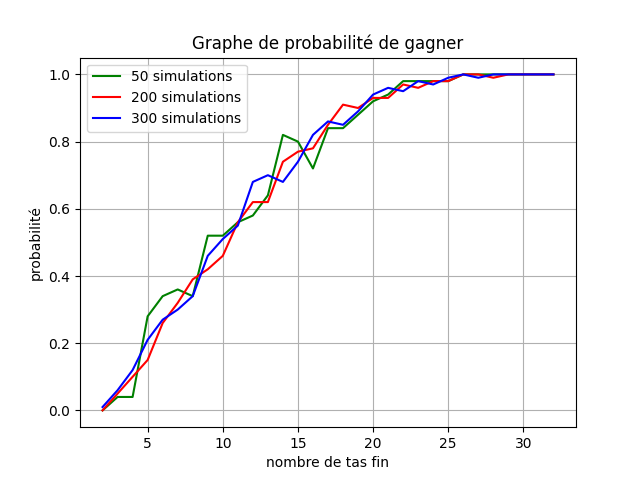
\includegraphics{graphe.png}}
\end{figure}

\par Nous remarquons ici que plus on autorise un plus grand nombre des tas final, plus la probabilité de gagner est grande. On constate aussi que la fin parfaite(2 tas) est vraiment difficile d'accès, puisque les graphes nous montre que sa probabilité est quasiment nulle.
\par En utilisant le module \emph{matplotlib}, voici comment on a pu réaliser le graphe dans la fonction principale:
	\\
	\begin{itemize}
	\color{blue}\item[•]Aperçu du code:
	\end{itemize}
	
	\lstset{language=Python}
	\lstset{frame=lines}
	\lstset{label={lst:code_direct}}
	\lstset{basicstyle=\footnotesize}
	\begin{lstlisting}
if __name__ == "__main__":

    x = linspace(2, 32, 31) #de 2 a 32, il y a 31 valeurs
    
    plt.figure()

    proba = stat_tout_nombre(50)
    proba1 = stat_tout_nombre(200)
    proba3 = stat_tout_nombre(300)

    y = []
    z = []
    w = []

    for a in proba:
        y.append(a)
    plt.plot(x,y, 'green')

    for a in proba1:
        z.append(a)
    plt.plot(x,z, 'red')

    for a in proba3:
        w.append(a)
    plt.plot(x,w, 'blue')

    plt.title("Graphe de probabilite de gagner")
    plt.xlabel("nombre de tas fin")
    plt.ylabel("probabilite")
    plt.legend(['50 simulations','200 simulations','300 simulations'])

    plt.grid()
    plt.show()
	\end{lstlisting}
\par Par ailleurs, l'on peut augmenter ces probabilités. C'est ce que l'on verra dans la partie suivante où l'on va tricher un peu dans ce jeu.


\end{document}